\subsection{Einsatzgebiete}

\begin{frame}{Architektur}
  \begin{columns}
    \column{.6\textwidth}
	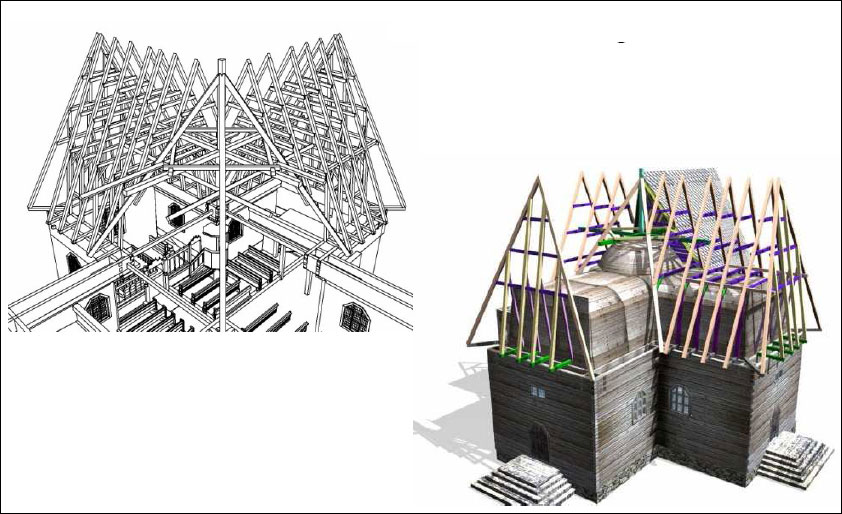
\includegraphics[width=0.9\textwidth]{../images/dach.jpg}
	\column{.4\textwidth}
	Abstrakte Landschaftsdarstellung in Bauplänen\\
	Quelle: Uni Rostock
  \end{columns}
\end{frame}

\begin{frame}{Medizin, Biologie}
  \begin{columns}
    \column{.6\textwidth}
	\includegraphics[width=\textwidth]<1>{../images/herz1.jpg}
	\includegraphics[width=\textwidth]<2->{../images/herz2.jpg}
	\column{.4\textwidth}
	Abstrakte Darstellung von Organismen\\
	Quelle: K. Hartmann, Magdeburg
  \end{columns}
\end{frame}

\begin{frame}{Spiele}
  \begin{columns}
    \column{.6\textwidth}
	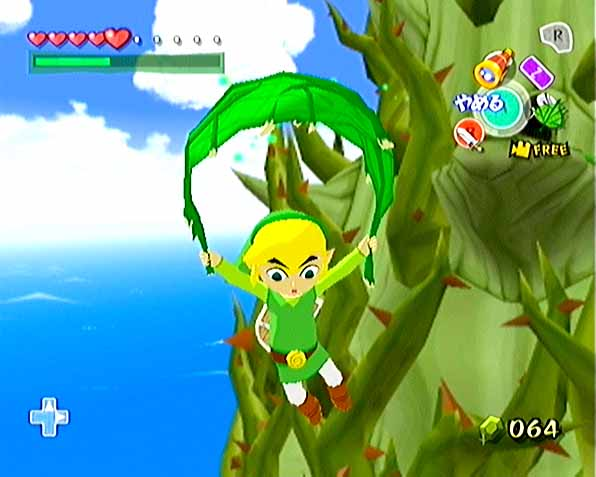
\includegraphics[width=\textwidth]{../images/Zelda.jpg}
	\column{.4\textwidth}
	Echtzeitdarstellung von comichaften Umgebungen\\
	Zelda, ein Nintendo-Spiel\\
	Quelle: Wikipedia
  \end{columns}
\end{frame}

\begin{frame}{Kunst}
  \begin{columns}
    \column{.6\textwidth}
	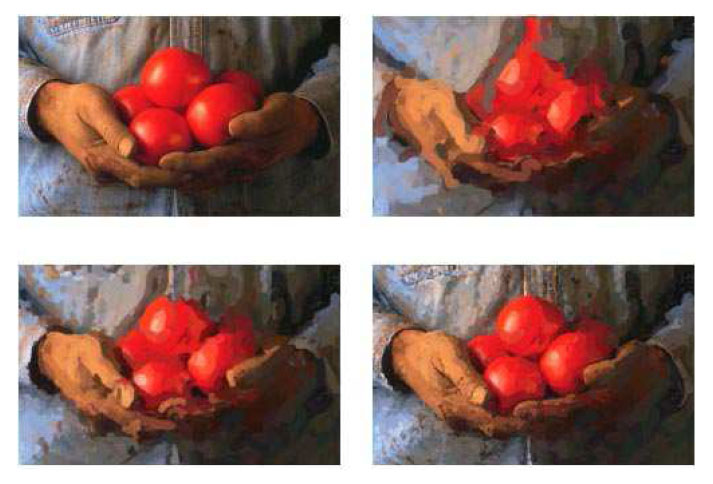
\includegraphics[width=\textwidth]{../images/kunscht.jpg}
	\column{.4\textwidth}
	Hervorhebung durch Verfälschung von Fotos\\
	Quelle: Uni Rostock
  \end{columns}
\end{frame}

\begin{frame}{Kartografie}
  \begin{columns}
    \column{.6\textwidth}
	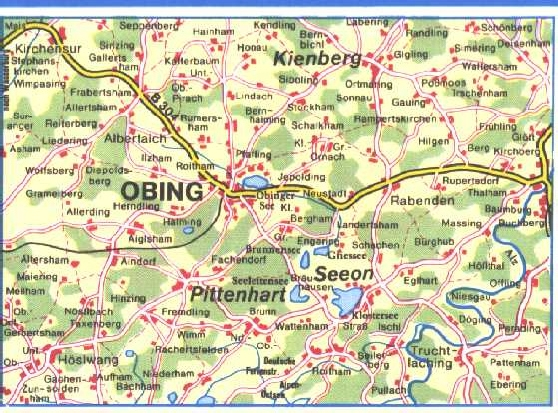
\includegraphics[width=\textwidth]{../images/landkarte.jpg}
	\column{.4\textwidth}
	Darstellung von Gewässern, Bewuchs und Schnee
  \end{columns}
\end{frame}

\begin{frame}{Maschinenbau}
  \begin{columns}
    \column{.6\textwidth}
	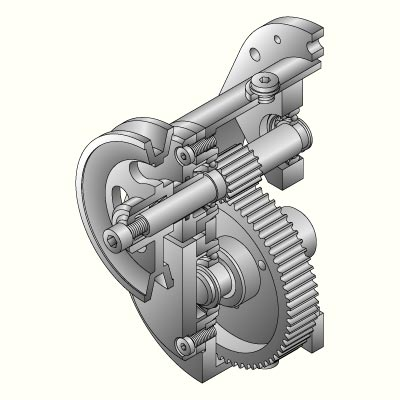
\includegraphics[width=0.9\textwidth]{../images/schnitt.jpg}
	\column{.4\textwidth}
	Vereinfachte technische Zeichnungen von Baugruppen\\
	Quelle: Gooch
  \end{columns}
\end{frame}